\section{Date: 2026-09-25}
\noindent \textbf{Series ID: CWSR0000SAE} 

\noindent This series is titled Consumer Price Index for All Urban Wage Earners and Clerical Workers: Education and Communication in U.S. City Average and has a frequency of Monthly. The units are Index Dec 1997=100 and the seasonal adjustment is Seasonally Adjusted.The observation start date is 1993-01-01 and the observation end date is 2026-08-01.The popularity of this series is 1. \\ 

\noindent \textbf{Series ID: LT65EXMNM35A647NCEN} 

\noindent This series is titled Total Tax Exemptions Under Age 65 for New Mexico and has a frequency of Annual. The units are Number of Exemptions and the seasonal adjustment is Not Seasonally Adjusted.The observation start date is 1989-01-01 and the observation end date is 2023-01-01.The popularity of this series is 1. \\ 

\subsection{Raw Regression}
\noindent Regresses the two series against each other directly. A significant result here can come just as easily from both series sharing a long-run trend as from any real relationship.

\begin{center}
\begin{tabular}{lclc}
\toprule
\textbf{Dep. Variable:}           & value\_fred\_LT65EXMNM35A647NCEN & \textbf{  R-squared:         } &     0.319   \\
\textbf{Model:}                   &               OLS                & \textbf{  Adj. R-squared:    } &     0.296   \\
\textbf{Method:}                  &          Least Squares           & \textbf{  F-statistic:       } &     13.61   \\
\textbf{Date:}                    &         Fri, 25 Sep 2026         & \textbf{  Prob (F-statistic):} &  0.000923   \\
\textbf{Time:}                    &             16:02:20             & \textbf{  Log-Likelihood:    } &   -383.39   \\
\textbf{No. Observations:}        &                  31              & \textbf{  AIC:               } &     770.8   \\
\textbf{Df Residuals:}            &                  29              & \textbf{  BIC:               } &     773.7   \\
\textbf{Df Model:}                &                   1              & \textbf{                     } &             \\
\textbf{Covariance Type:}         &            nonrobust             & \textbf{                     } &             \\
\bottomrule
\end{tabular}
\begin{tabular}{lcccccc}
                                  & \textbf{coef} & \textbf{std err} & \textbf{t} & \textbf{P$> |$t$|$} & \textbf{[0.025} & \textbf{0.975]}  \\
\midrule
\textbf{const}                    &    1.111e+06  &     8.56e+04     &    12.985  &         0.000        &     9.36e+05    &     1.29e+06     \\
\textbf{value\_fred\_CWSR0000SAE} &    2729.6493  &      739.846     &     3.689  &         0.001        &     1216.494    &     4242.805     \\
\bottomrule
\end{tabular}
\begin{tabular}{lclc}
\textbf{Omnibus:}       &  1.749 & \textbf{  Durbin-Watson:     } &    0.439  \\
\textbf{Prob(Omnibus):} &  0.417 & \textbf{  Jarque-Bera (JB):  } &    1.177  \\
\textbf{Skew:}          &  0.477 & \textbf{  Prob(JB):          } &    0.555  \\
\textbf{Kurtosis:}      &  2.985 & \textbf{  Cond. No.          } &     937.  \\
\bottomrule
\end{tabular}
%\caption{OLS Regression Results}
\end{center}

Notes: \newline
 [1] Standard Errors assume that the covariance matrix of the errors is correctly specified.

\begin{figure}
\centering
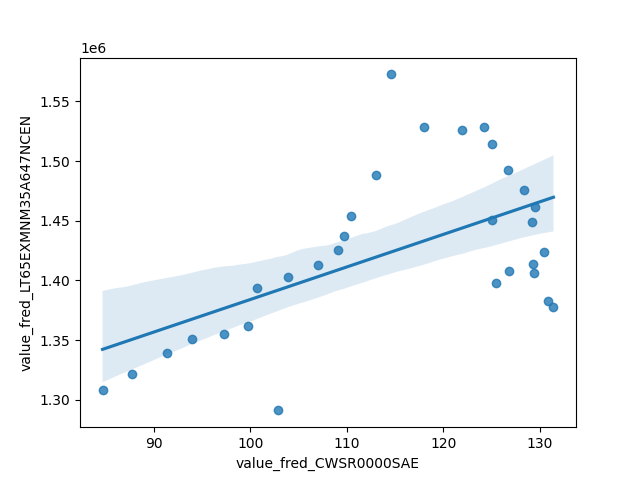
\includegraphics[scale = 0.9]{plots/plot_2026-09-25.png}
\caption{Raw Regression Plot for 2026-09-25}
\end{figure}
\newpage
\subsection{Detrended Regression}
\noindent Regresses the residuals of each series after removing its own linear time trend, so a shared trend can no longer drive the result on its own. A relationship that stays significant here is better evidence of a genuine link between the two series.

\begin{center}
\begin{tabular}{lclc}
\toprule
\textbf{Dep. Variable:}                      & value\_fred\_LT65EXMNM35A647NCEN\_detrended & \textbf{  R-squared:         } &     0.508   \\
\textbf{Model:}                              &                     OLS                     & \textbf{  Adj. R-squared:    } &     0.491   \\
\textbf{Method:}                             &                Least Squares                & \textbf{  F-statistic:       } &     29.99   \\
\textbf{Date:}                               &               Fri, 25 Sep 2026              & \textbf{  Prob (F-statistic):} &  6.75e-06   \\
\textbf{Time:}                               &                   16:02:20                  & \textbf{  Log-Likelihood:    } &   -375.82   \\
\textbf{No. Observations:}                   &                        31                   & \textbf{  AIC:               } &     755.6   \\
\textbf{Df Residuals:}                       &                        29                   & \textbf{  BIC:               } &     758.5   \\
\textbf{Df Model:}                           &                         1                   & \textbf{                     } &             \\
\textbf{Covariance Type:}                    &                  nonrobust                  & \textbf{                     } &             \\
\bottomrule
\end{tabular}
\begin{tabular}{lcccccc}
                                             & \textbf{coef} & \textbf{std err} & \textbf{t} & \textbf{P$> |$t$|$} & \textbf{[0.025} & \textbf{0.975]}  \\
\midrule
\textbf{const}                               &    4.538e-09  &     8271.954     &  5.49e-13  &         1.000        &    -1.69e+04    &     1.69e+04     \\
\textbf{value\_fred\_CWSR0000SAE\_detrended} &    1.073e+04  &     1959.312     &     5.477  &         0.000        &     6722.977    &     1.47e+04     \\
\bottomrule
\end{tabular}
\begin{tabular}{lclc}
\textbf{Omnibus:}       &  6.655 & \textbf{  Durbin-Watson:     } &    0.863  \\
\textbf{Prob(Omnibus):} &  0.036 & \textbf{  Jarque-Bera (JB):  } &    6.187  \\
\textbf{Skew:}          &  0.543 & \textbf{  Prob(JB):          } &   0.0453  \\
\textbf{Kurtosis:}      &  4.900 & \textbf{  Cond. No.          } &     4.22  \\
\bottomrule
\end{tabular}
%\caption{OLS Regression Results}
\end{center}

Notes: \newline
 [1] Standard Errors assume that the covariance matrix of the errors is correctly specified.

\begin{figure}
\centering
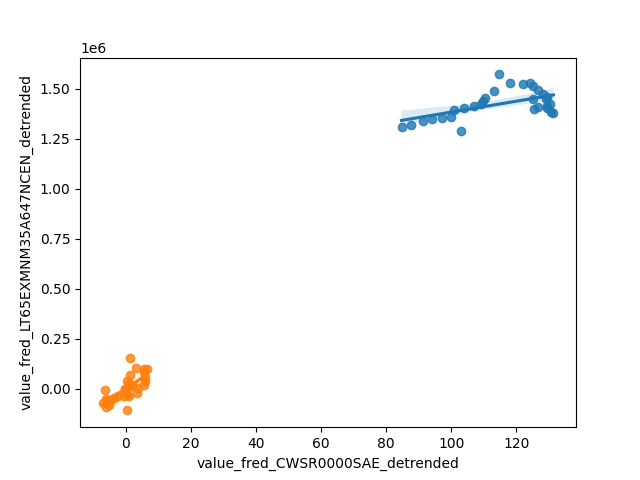
\includegraphics[scale = 0.9]{plots/plot_2026-09-25_detrended.png}
\caption{Detrended Regression Plot for 2026-09-25}
\end{figure}
\newpage
